\documentclass[11pt]{article}
\usepackage[margin=1in]{geometry}
\usepackage{graphicx}
\graphicspath{{images/}{../images/}{report/images/}}
\usepackage{listings}
\usepackage{xcolor}
\usepackage{amsmath}
\usepackage{booktabs}
\usepackage{enumitem}
\usepackage[hidelinks]{hyperref}
\setcounter{tocdepth}{2}

% SystemVerilog code styling
\lstdefinestyle{verilog}{
    language=Verilog,
    basicstyle=\ttfamily\small,
    keywordstyle=\color{blue}\bfseries,
    commentstyle=\color{green!60!black},
    stringstyle=\color{red},
    numbers=left,
    numberstyle=\tiny\color{gray},
    stepnumber=1,
    numbersep=8pt,
    backgroundcolor=\color{gray!5},
    frame=single,
    breaklines=true,
    breakatwhitespace=false,
    captionpos=b,
    tabsize=2
}

\title{Project 3: Reorder Buffer Extension to a\\2-Wide Superscalar Tomasulo CPU}
\author{Sangeeth Thayaaparan \\ RIN: 662037988}
\date{\today}

\begin{document}

\maketitle

\begin{center}
  \large\textbf{Tools:} ModelSim -- Intel FPGA Starter Edition 2020.1, SystemVerilog RTL
\end{center}

\begin{abstract}
  This report documents the Project 3 extension of my previously-submitted 2-wide
  superscalar Tomasulo CPU. The baseline design --- in-order dispatch, three
  reservation stations, pipelined functional units, and tag-based forwarding over a
  Common Data Bus (CDB) --- is retained. On top of it I added a 16-entry Reorder
  Buffer (ROB) that guarantees in-order \emph{commit} of instructions that are
  dispatched in order but execute and write their results back out of order. The
  ROB entry index now doubles as the rename tag used throughout the pipeline, so
  the existing CDB and RS snoop logic required no semantic change --- only a
  widening of the tag field from 3 to 4 bits. The extension adds (i) an ROB
  module with in-order commit, (ii) predict-not-taken branch handling with
  single-cycle blanket flush on misprediction, (iii) a one-entry store buffer
  that forwards stores-in-flight to younger loads so memory writes can be deferred
  to commit without serialising load/store traffic, and (iv) a precise-exception
  path triggered by misaligned load/store addresses. All eleven regression tests
  (seven Tomasulo baselines and four new ROB/exception tests) pass in ModelSim.
\end{abstract}

\tableofcontents
\listoffigures
\listoftables

\newpage

\section{What Changed Relative to Project 2}
\label{sec:what_changed}

The Project 2 submission implemented the Tomasulo algorithm but committed results
to the architectural register file on the same cycle they appeared on the CDB.
That is functionally correct for a workload with no branches and no exceptions,
but it does not preserve a precise architectural state: a speculative instruction
could retire before it was known to be on the correct path.  Project 3 adds the
missing in-order commit stage, backed by a Reorder Buffer.  The concrete
edits made to the existing codebase are summarised below.

\begin{table}[h]
  \centering
  \small
  \begin{tabular}{p{3.4cm} p{11.5cm}}
    \toprule
    \textbf{File}                            & \textbf{Change}                                                                                                                              \\
    \midrule
    \texttt{rob.sv}                          & New module. 16-entry circular queue, ROB index is the rename tag.                                                                            \\
    \texttt{datapath.sv}                     & ROB instantiated; tags now come from the ROB rather than an internal counter. One-entry store buffer added.
    Architectural-register write and memory-store write both gated on \texttt{commitV}. Flush signal broadcast to all stateful modules.                                                     \\
    \texttt{rat.sv}                          & Pending tag is cleared on \emph{commit}, not on CDB broadcast. Added \texttt{flush} input.                                                   \\
    \texttt{rs.sv}                           & Added \texttt{flush} input; LS station parameterised with \texttt{INORDER=1}.                                                                \\
    \texttt{fu\_pipe.sv}, \texttt{fu\_ls.sv} & Added \texttt{flush} input that clears in-flight state. \texttt{fu\_ls} also detects misaligned addresses and raises a new exception signal. \\
    \texttt{ifetch.sv}                       & Added \texttt{flush}/\texttt{flushPC} inputs; on flush the PC is redirected to the ROB-reported target.                                      \\
    \texttt{dispatchunit.sv}                 & Added \texttt{flush} input that suppresses dispatch for the redirect cycle.                                                                  \\
    \texttt{tdecode.sv}                      & Added decoding for \texttt{beq} (B-type) and a new \texttt{isBranch} output.                                                                 \\
    \texttt{testbench.sv}                    & Monitors a new \texttt{trap}/\texttt{trapPC} output for precise-exception tests.                                                             \\
    \bottomrule
  \end{tabular}
  \caption{Summary of files modified from the Project 2 submission.}
  \label{tbl:diff}
\end{table}

\noindent\textbf{Assumptions for this extension (justified in the rubric's ``reasonable
  assumptions'' clause):}
\begin{itemize}[noitemsep]
  \item Only \texttt{beq} is added to the branch ISA. The flush/redirect mechanism
        is fully general; extending decode to \texttt{bne/blt/bge/bltu/bgeu} is
        a $\leq$10-line change to \texttt{tdecode.sv} if needed.
  \item Branch prediction is ``always not-taken''. The spec's reach goal of a
        two-level adaptive predictor is not pursued.
  \item Precise exceptions are demonstrated with a single exception class ---
        address misalignment on loads and stores --- because the base ISA has no
        arithmetic traps (no division) and no explicit trap instruction.
\end{itemize}

\section{Specification and Rationale}

\subsection{Instruction Set Architecture (ISA) Subset}

The processor supports a minimal subset of RISC-V 32-bit instructions:

\begin{itemize}[noitemsep]
  \item \textbf{Immediate (I-type)}: \texttt{addi}
  \item \textbf{Register (R-type)}: \texttt{add}, \texttt{mul}
  \item \textbf{Store (S-type)}: \texttt{sw}
  \item \textbf{Load (I-type variant)}: \texttt{lw}
  \item \textbf{Branch (B-type)} \emph{(new in Project 3)}: \texttt{beq}
  \item \textbf{Special}: \texttt{nop} (encoded as \texttt{addi x0, x0, 0})
\end{itemize}

\textbf{Out-of-scope}: other branches, jumps, floating point, CSRs, and cache
coherence (single core).

\subsection{Microarchitecture Parameters}

\begin{table}[h]
  \centering
  \begin{tabular}{ll}
    \toprule
    \textbf{Parameter}                  & \textbf{Value}                       \\
    \midrule
    Dispatch width                      & 2 instructions/cycle                 \\
    Rename tag width (\texttt{TAGW})    & 4 bits (was 3 in Project 2)          \\
    In-flight tag space                 & 16 \emph{(= ROB depth; was 8)}       \\
    Reservation Station depths          & ADD: 4, MUL: 3, LS: 4                \\
    LS reservation station              & \texttt{INORDER=1} (strict in-order) \\
    \midrule
    \textbf{Functional Unit Latencies:} &                                      \\
    ADD / \texttt{BEQ} (shared ADD FU)  & 4 cycles                             \\
    MUL                                 & 6 cycles                             \\
    LS                                  & 2 cycles (address gen + access)      \\
    \midrule
    Reorder Buffer (ROB) depth          & 16 entries                           \\
    Store buffer                        & 1 entry                              \\
    Register Alias Table entries        & 32 (RISC-V)                          \\
    Memory size (unified)               & 4,096 words (16 KB)                  \\
    \bottomrule
  \end{tabular}
  \caption{Key microarchitecture parameters (Project 3).}
  \label{tbl:arch_params}
\end{table}

\subsection{Design Decisions}

\begin{itemize}[noitemsep]
  \item \textbf{ROB index == rename tag.} The obvious alternative is a separate
        physical-register file with its own tag space. Folding the two into one
        saves the tag-to-rob lookup at commit and keeps the Project 2 CDB /
        RS snoop logic unchanged.
  \item \textbf{Predict not-taken, resolve at commit.} The fetch unit always
        fetches \texttt{PC+4}. When a taken branch reaches the ROB head, the ROB
        raises a one-cycle flush that synchronously resets the RAT, every RS,
        every FU, the ifetch queue, the dispatch unit, the store buffer, and the
        ROB itself, then redirects fetch to the branch target.
  \item \textbf{RAT cleared on commit, not on CDB.} In Project 2 the RAT's
        pending-tag bit was cleared as soon as the producer's result was
        broadcast on the CDB. With a ROB this is too early: the writeback is
        still speculative. The RAT now clears only when the instruction retires
        through the ROB, which means a reader dispatched after the producer
        completes but before it commits still sees the tag, not the final
        value --- correct behaviour under speculation.
  \item \textbf{INORDER LS reservation station.} With the ROB deferring stores to
        commit time, a younger load must not bypass an older store in the RS, or
        it will miss the store's data. Setting \texttt{INORDER=1} on the LS RS
        forces the oldest entry to issue first (the ADD and MUL RSes remain
        out-of-order).
  \item \textbf{One-entry store buffer.} Even with in-order LS issue, a store
        writes memory only at commit, so a load that follows it into the LS FU
        could read stale RAM. The store buffer captures
        \{\texttt{addr},\texttt{data}\} at the moment the store executes and
        forwards to a matching load; it drains to RAM on commit and is cleared
        on flush. Capacity 1 is sufficient because the LS RS issues in order and
        the LS FU only holds one in-flight store.
  \item \textbf{Precise exceptions.} Every ROB entry carries an \texttt{exc} bit.
        The LS FU sets it, via a dedicated writeback port on the ROB, whenever
        the effective address is not word-aligned. Commit refuses to retire an
        entry whose \texttt{exc} bit is set and instead raises a top-level
        \texttt{trap} signal. Because older entries have already committed and
        younger ones are blocked behind the trapping entry, the architectural
        state at the trap point is precise.
\end{itemize}

\subsection{System Architecture}

Figure~\ref{fig:pipeline_architecture} is the original Project 2 pipeline view.
For Project 3, the architectural change is conceptually simple but critical:
the ROB inserts an in-order commit stage after writeback and broadcasts
flush/redirect control back to all speculative state on misprediction. The
fetch/decode/rename/dispatch/issue/execute/CDB path remains unchanged.

\begin{figure}[!htbp]
  \centering
  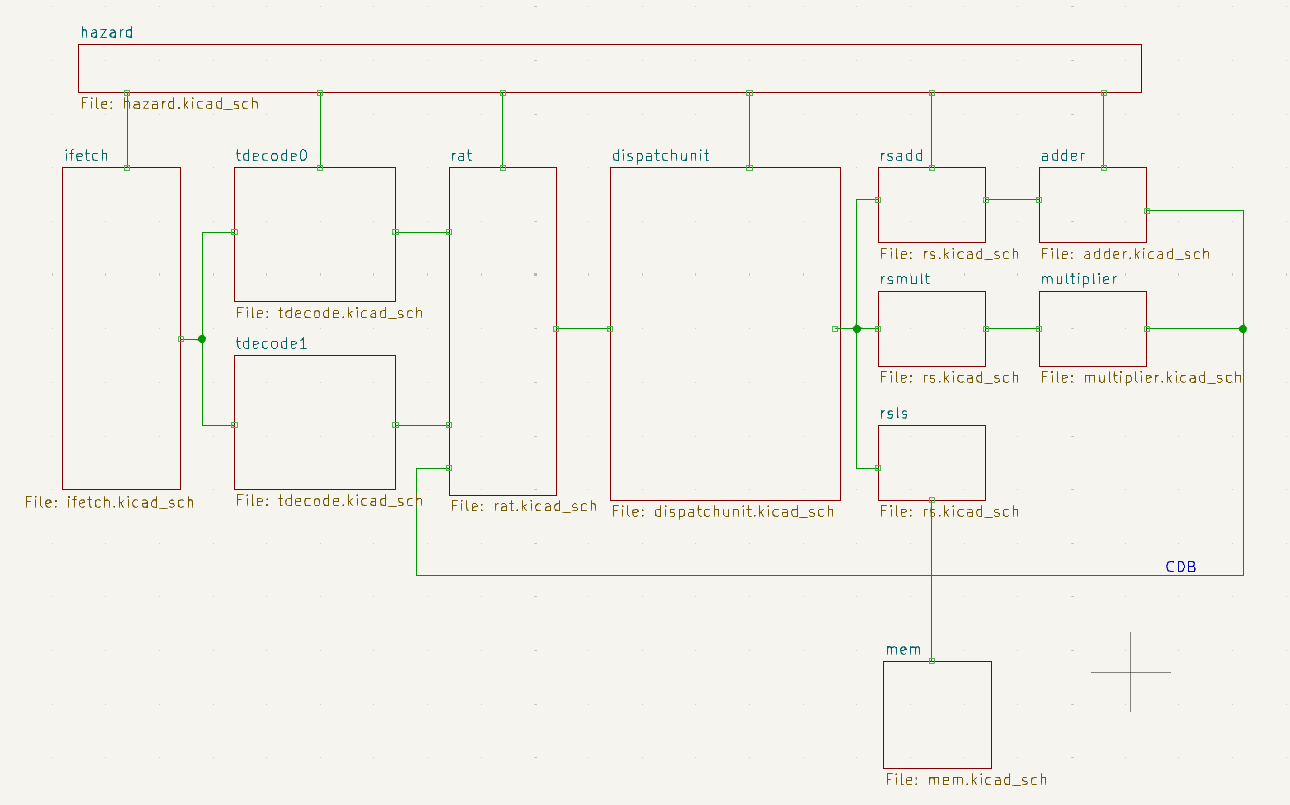
\includegraphics[width=0.95\textwidth]{images/SuperscalarCPU_Archiecture.png}
  \caption{Baseline Tomasulo pipeline from Project 2. Project 3 inserts a ROB
    commit stage after the CDB and adds a flush fan-out from the ROB back to
    every stateful module.}
  \label{fig:pipeline_architecture}
\end{figure}

\begin{figure}[!htbp]
  \centering
  \IfFileExists{images/SuperscalarCPU_ROB_Architecture.png}{%
    \includegraphics[width=0.95\textwidth]{images/SuperscalarCPU_ROB_Architecture.png}%
  }{%
    \fbox{\parbox{0.92\textwidth}{\centering
        \vspace{1.8cm}
        Insert updated architecture diagram here:\\
        Project 3 pipeline with ROB commit stage, branch flush fan-out, and
        store-buffer forwarding path.
        \vspace{1.8cm}
      }}%
  }
  \caption{Updated Project 3 architecture diagram (ROB-aware view).}
  \label{fig:pipeline_architecture_rob}
\end{figure}

\section{The Reorder Buffer}
\label{sec:rob}

\subsection{Entry Format}

Each ROB entry is a packed struct containing the fields the rubric requires:

\begin{table}[h]
  \centering
  \small
  \begin{tabular}{p{3cm} p{2cm} p{9cm}}
    \toprule
    \textbf{Field}        & \textbf{Width} & \textbf{Purpose}                                                                                                     \\
    \midrule
    \texttt{valid}        & 1 bit          & Entry occupies a ROB slot.                                                                                           \\
    \texttt{done}         & 1 bit          & Instruction has written its result back (CDB for ALU/load, \texttt{storeDoneV} for store, \texttt{excV} for a trap). \\
    \texttt{exc}          & 1 bit          & Exception occurred during execution (misaligned address).                                                            \\
    \texttt{isBranch}     & 1 bit          & Branch; at commit, inspect \texttt{result[0]} to decide flush.                                                       \\
    \texttt{isStore}      & 1 bit          & Store; at commit, drain the store buffer entry to RAM.                                                               \\
    \texttt{regw}         & 1 bit          & Instruction writes an architectural register.                                                                        \\
    \texttt{rd}           & 5 bits         & Destination register index.                                                                                          \\
    \texttt{result}       & 32 bits        & CDB result (ALU / load value, branch-taken flag).                                                                    \\
    \texttt{storeAddr}    & 32 bits        & Captured store address (for commit-time RAM write).                                                                  \\
    \texttt{storeData}    & 32 bits        & Captured store data.                                                                                                 \\
    \texttt{branchTarget} & 32 bits        & PC to redirect to on misprediction.                                                                                  \\
    \texttt{pc}           & 32 bits        & Dispatch-time PC (reported with a trap).                                                                             \\
    \bottomrule
  \end{tabular}
  \caption{ROB entry fields. Covers every field enumerated in the rubric:
    instruction type (flags), destination (\texttt{rd}), completion
    status (\texttt{done}), exception status (\texttt{exc}), and
    implementation fields.}
  \label{tbl:rob_entry}
\end{table}

\paragraph{Why no ``operands'' field.} The rubric lists ``instruction type and
operands'' among the ROB fields. In a Tomasulo design, operand \emph{values}
are consumed at dispatch by the reservation stations and never re-read by the
ROB; the ROB stores only the \emph{result}. This is the standard split between
RS (operand wait) and ROB (in-order retirement). The ROB does retain the
fields required to roll the pipeline back to a precise architectural state on
flush: destination register, result, and PC.

\subsection{Dispatch: ROB Entry Allocation (Rubric Item 3)}

Tags are allocated combinationally from the current tail pointer:

\begin{lstlisting}[style=verilog, caption=Two-wide ROB tag allocation]
assign enq0tag = tail;
assign enq1tag = enq0v ? (tail + TAGW'(1)) : tail;
assign robFull = (count >= 5'(DEPTH - 1));
\end{lstlisting}

The datapath uses these tags as \emph{rename} tags for the RAT and as
destination tags for the reservation stations. \texttt{robFull} participates in
dispatch gating so a full ROB stalls the front-end:

\begin{lstlisting}[style=verilog, caption=ROB full participates in dispatch gating (datapath.sv)]
assign can0Eff = can0Haz && !robFull;
assign can1Eff = can1Haz && !robFull;
\end{lstlisting}

NOPs do not consume ROB slots (\texttt{enq0v = dispatch0 \&\& !nop0}); this was
a deliberate choice to keep the tag space small. An ADD/MUL entry is allocated
with \texttt{done=0}; a \texttt{nop}-like instruction with no architectural
effect (no register write, no store, not a branch) is allocated with
\texttt{done=1} so it retires on the next commit cycle without waiting for a
CDB broadcast.

\subsection{Update on Completion (Rubric Item 4)}

Three completion ports feed the ROB:

\begin{lstlisting}[style=verilog, caption=ROB writeback from CDB / store FU / exception]
// CDB: arithmetic and loads
if (cdbv && entries[cdbt].valid && !entries[cdbt].done)
    entries[cdbt].done <= 1'b1;
if (cdbv && entries[cdbt].valid)
    entries[cdbt].result <= cdbr;

// Store FU writeback (address + data captured at execute)
if (storeDoneV && entries[storeDoneTag].valid && !entries[storeDoneTag].done) begin
    entries[storeDoneTag].done      <= 1'b1;
    entries[storeDoneTag].storeAddr <= storeDoneAddr;
    entries[storeDoneTag].storeData <= storeDoneData;
end

// Exception port (misaligned LW/SW)
if (excV && entries[excTag].valid && !entries[excTag].done) begin
    entries[excTag].done <= 1'b1;
    entries[excTag].exc  <= 1'b1;
end
\end{lstlisting}

\subsection{Commit Stage (Rubric Item 5)}

The commit logic is a combinational head check that fans out to (i) RAT
clear, (ii) architectural register write, (iii) memory write, and (iv)
branch-flush or trap generation:

\begin{lstlisting}[style=verilog, caption=ROB commit logic]
if (entries[head].valid && entries[head].done) begin
    if (entries[head].exc) begin
        trap   = 1'b1;
        trapPC = entries[head].pc;
    end else begin
        commitV         = 1'b1;
        commitRd        = entries[head].rd;
        commitResult    = entries[head].result;
        commitRegW      = entries[head].regw;
        commitIsStore   = entries[head].isStore;
        commitStoreAddr = entries[head].storeAddr;
        commitStoreData = entries[head].storeData;

        // Predict not-taken: result[0]=1 => branch was actually taken => mispredict
        if (entries[head].isBranch && entries[head].result[0]) begin
            flush   = 1'b1;
            flushPC = entries[head].branchTarget;
        end
    end
end
\end{lstlisting}

On a successful commit the head advances and the entry's \texttt{valid} bit is
cleared. The datapath gates both \texttt{areg[commitRd] <= commitResult} and
\texttt{MemWrite = commitV \&\& commitIsStore} on this single commit signal, so
no speculative instruction ever modifies architectural state.

\subsection{Branch Misprediction and Flush (Rubric Item 6)}

Branches are routed through the ADD functional unit. The \texttt{dispStore}
bit on the ADD RS entry is repurposed as \texttt{isBranch}; at issue, the ADD
datapath computes \texttt{(rs1 == rs2) ? 1 : 0} instead of \texttt{rs1 + rs2}
when the bit is set. The result bit therefore rides the CDB into the ROB entry
alongside non-branch results, and the commit stage does a single bit-0 test.

On \texttt{flush} the ROB, RAT, all three RSes, both pipelined FUs, the LS FU,
the ifetch queue, the dispatch unit, and the store buffer all reset their state
synchronously on the next clock edge (single-cycle blanket flush). Fetch
redirects to \texttt{flushPC}; dispatch is suppressed for the redirect cycle.
Because the RAT is re-zeroed, any register read by the first instruction after
the flush sees the architectural value in \texttt{areg}, which was brought
up-to-date by the older committed instructions.

\subsection{Precise Exceptions (Rubric Target Goal, 100 tier)}
\label{sec:precise_exc}

The LS functional unit flags any computed address whose low two bits are
non-zero:

\begin{lstlisting}[style=verilog, caption=Misaligned-address detection in fu\_ls]
logic misaligned;
assign misaligned = (a0[1:0] != 2'b00);

if (v0) begin
    if (misaligned) begin
        excV   <= 1'b1;
        excTag <= t0;      // suppress load/store memory access this cycle
    end else if (st0) begin ...storeDoneV path... end
    else        begin ...loadDoneV path... end
end
\end{lstlisting}

The ROB receives \texttt{excV}/\texttt{excTag}, marks the entry
\texttt{done=1, exc=1}, and refuses to commit it. Because ROB commit is
strictly in-order, older instructions still retire normally, while the
trapping entry blocks every younger instruction from modifying architectural
state --- the rubric's precise-exception criterion. The test bench exposes
a top-level \texttt{trap}/\texttt{trapPC} signal and prints
\texttt{TRAP\_SIGNATURE: trapPC=...} when it fires. Test
\texttt{rob04\_misaligned\_trap} (Section~\ref{sec:test_rob04}) exercises this
path.

\section{Modified and New Modules}

This section documents only the modules that changed, and the one new module.
Unchanged modules (ifetch queue logic, tdecode except for BEQ, dispatchpack,
rsarbiter, fu\_pipe ALU functionality, cdb, mem) are covered in the Project 2
submission and not repeated here.

\subsection{Module: rob (new)}

\paragraph{Behaviour.}
16-entry circular queue of ROB entries. Head/tail pointers are
\texttt{TAGW}-bit counters; \texttt{count} tracks occupancy. Two enqueue ports
(one per dispatch slot), three writeback ports (CDB, store FU, exception), one
commit port, and flush/trap outputs.

\paragraph{Key state.}
\texttt{entries[16]}, \texttt{head}, \texttt{tail}, \texttt{count}. On reset or
flush every entry's \texttt{valid} is cleared and pointers reset to zero.

\paragraph{Interface (abridged).}
\begin{lstlisting}[style=verilog, caption=rob.sv port list (abridged)]
module rob #(parameter int DEPTH=16, parameter int TAGW=4)(
    input  logic clk, reset,
    // Dispatch (two-wide)
    input  logic            enq0v, enq1v,
    input  logic [4:0]      enq0rd, enq1rd,
    input  logic            enq0regw, enq0isStore, enq0isBranch,
    input  logic            enq1regw, enq1isStore, enq1isBranch,
    input  logic [31:0]     enq0branchTarget, enq0pc,
    input  logic [31:0]     enq1branchTarget, enq1pc,
    output logic [TAGW-1:0] enq0tag, enq1tag,
    output logic            robFull,
    // Writeback
    input  logic            cdbv, input logic [TAGW-1:0] cdbt, input logic [31:0] cdbr,
    input  logic            storeDoneV, input logic [TAGW-1:0] storeDoneTag,
    input  logic [31:0]     storeDoneAddr, storeDoneData,
    input  logic            excV, input logic [TAGW-1:0] excTag,
    // Commit
    output logic            commitV, commitRegW, commitIsStore,
    output logic [4:0]      commitRd,
    output logic [TAGW-1:0] commitTag,
    output logic [31:0]     commitResult, commitStoreAddr, commitStoreData,
    // Pipeline-wide signals
    output logic            flush,  output logic [31:0] flushPC,
    output logic            trap,   output logic [31:0] trapPC
);
\end{lstlisting}

\subsection{Module: rat (modified)}

The pending-tag clear has moved from CDB writeback to ROB commit. A new
\texttt{flush} input clears every \texttt{valid} bit synchronously on
misprediction.

\begin{lstlisting}[style=verilog, caption=RAT writeback (commit-time clear + flush)]
always_ff @(posedge clk or posedge reset) begin
  if (reset || flush) begin
    for (int i = 0; i < 32; i++) valid[i] <= 1'b0;
  end else begin
    // ... rename0/rename1 updates ...
    if (clearv && clearrd != 5'b0 && tag[clearrd] == cleartag)
      valid[clearrd] <= 1'b0;  // driven by commitV/commitRd/commitTag from ROB
  end
end
\end{lstlisting}

\subsection{Module: rs (modified)}

A new \texttt{flush} input clears every entry on misprediction. An
\texttt{INORDER} parameter was added; when set to 1 (LS station) the RS will
only issue its oldest busy entry, even if a younger entry is ready.

\subsection{Module: fu\_pipe and fu\_ls (modified)}

Both receive a \texttt{flush} input that zeroes in-flight stage state. The LS
unit additionally raises \texttt{excV}/\texttt{excTag} on misaligned effective
addresses (Section~\ref{sec:precise_exc}); in this case \texttt{loadDoneV} /
\texttt{storeDoneV} are \emph{not} asserted, so memory is not accessed.

\subsection{Module: ifetch (modified)}

A \texttt{flush} input redirects the PC to a new target on the same cycle the
ROB detects a misprediction:

\begin{lstlisting}[style=verilog, caption=ifetch redirect on flush]
always_ff @(posedge clk) begin
  if (reset)       head <= '0;
  else if (flush)  head <= flushPC[QW+1:2];
  else             head <= head + pop;
end
\end{lstlisting}

\subsection{Module: dispatchunit (modified)}

A \texttt{flush} input forces \texttt{dispatch0=dispatch1=iqpop=0} for the
redirect cycle, so the pipeline does not try to push the instructions that
were in the queue when the flush fired.

\subsection{Module: tdecode (modified)}

B-type decoding for \texttt{beq} was added. The immediate follows the RISC-V
B-type layout. The new \texttt{isBranch} output is carried through
\texttt{dispatchpack} and into the ADD reservation station, where the
\texttt{dispStore} bit is reused as an ``is-branch'' marker for instructions
routed to the ADD FU.

\begin{lstlisting}[style=verilog, caption=BEQ decode]
end else if ((opc == 7'b1100011) && (f3 == 3'b000)) begin
    op = OPBEQ; kind = KADD; regw = 1'b0; isBranch = 1'b1; rd = 5'b0;
    imm = {{19{instr[31]}}, instr[31], instr[7], instr[30:25], instr[11:8], 1'b0};
end
\end{lstlisting}

\subsection{Store buffer (new, in datapath)}

A single register set $\{\texttt{stbufValid}, \texttt{stbufAddr},
  \texttt{stbufData}\}$ captures the output of the LS FU on
\texttt{storeDoneV}. A combinational forwarding mux intercepts the load
data feeding the CDB:

\begin{lstlisting}[style=verilog, caption=Store-buffer update and forwarding]
always_ff @(posedge clk or posedge reset) begin
  if (reset || robFlush) begin
    stbufValid <= 1'b0;
  end else begin
    if (storeDoneV) begin
      stbufValid <= 1'b1;
      stbufAddr  <= storeDoneAddr;
      stbufData  <= storeDoneData;
    end
    if (commitV && commitIsStore) stbufValid <= 1'b0;
  end
end

assign loadResult = (stbufValid && loadDoneV && (stbufAddr == loadAddr))
                  ? stbufData : ReadDataM;
// cdb0.ldr <= loadResult
\end{lstlisting}

\subsection{Testbench (modified)}

The test harness now samples both signature paths: a word store to address 100
(\texttt{FINAL\_SIGNATURE}) and the ROB trap (\texttt{TRAP\_SIGNATURE}). Either
terminates the simulation.

\section{Verification and Results}

Eleven tests are run through the ModelSim regression harness.
\texttt{tests/run\_tomasulo\_modelsim\_suite.sh} compiles the design and sweeps
every \texttt{.mem} image, comparing the captured signature against the
expected value.

\subsection{Suite Summary}

\begin{table}[h]
  \centering
  \small
  \begin{tabular}{l l l l}
    \toprule
    \textbf{Test}                          & \textbf{What it exercises}                           & \textbf{Expected} & \textbf{Result} \\
    \midrule
    \texttt{tomasulo01\_addi\_smoke}       & ADDI + SW smoke path                                 & 5                 & PASS            \\
    \texttt{tomasulo02\_add\_chain}        & RAW dep resolved through CDB                         & 21                & PASS            \\
    \texttt{tomasulo03\_mul\_basic}        & 6-cycle MUL FU                                       & 42                & PASS            \\
    \texttt{tomasulo04\_sw\_lw\_roundtrip} & SW/LW roundtrip at the same address                  & 33                & PASS            \\
    \texttt{tomasulo05\_dual\_independent} & Two independent ADDIs dispatched together            & 11                & PASS            \\
    \texttt{tomasulo06\_slot\_dep}         & Same-cycle slot0$\to$slot1 RAW tag injection         & 9                 & PASS            \\
    \texttt{tomasulo07\_mul\_add\_mix}     & MUL and ADD overlap on separate FUs                  & 17                & PASS            \\
    \midrule
    \texttt{rob01\_waw\_order}             & WAW: fast ADDI retires \emph{after} slow MUL via ROB & 99                & PASS            \\
    \texttt{rob02\_beq\_not\_taken}        & BEQ correct prediction (predict-not-taken)           & 43                & PASS            \\
    \texttt{rob03\_beq\_taken}             & BEQ misprediction, full pipeline flush + redirect    & 77                & PASS            \\
    \texttt{rob04\_misaligned\_trap}       & Precise exception on misaligned LW                   & \texttt{trapPC=8} & PASS            \\
    \bottomrule
  \end{tabular}
  \caption{ModelSim regression results (11/11 passing).}
  \label{tbl:suite_results}
\end{table}

The seven Tomasulo baseline tests were carried over from Project 2 and still
pass, confirming that adding the ROB did not regress the out-of-order core.
The four new tests target the Project 3 features directly and are described
below.

\subsection{Test: rob01\_waw\_order}

\paragraph{Purpose.}
Demonstrates that in-order commit preserves the correct
final architectural state under a write-after-write (WAW) hazard with
asymmetric FU latencies.

\paragraph{Stimulus.}
\begin{lstlisting}[style=verilog, caption=WAW ordering (rob01\_waw\_order.s)]
addi x2, x0, 6
addi x3, x0, 7
mul  x1, x2, x3     ; slow: x1 <= 42 via 6-cycle MUL
addi x1, x0, 99     ; fast: x1 <= 99 via 4-cycle ADD (but dispatched AFTER the MUL)
sw   x1, 100(x0)    ; must observe 99, not 42
\end{lstlisting}

\paragraph{Expected.}
The ADDI completes \emph{before} the MUL on the FU side, but dispatch order
assigns the MUL a smaller ROB tag. The RAT therefore maps \texttt{x1} to the
ADDI's tag (the most recent writer). The SW uses the ADDI's tag as its source.
At commit, the ROB retires the MUL first (updating \texttt{areg[x1]=42} and
being immediately overwritten at commit of the ADDI to 99). The SW sees the
ADDI's result through CDB snoop in the RS and stores 99. Expected signature
99.

\paragraph{Result.} Signature 99 captured. PASS.

\subsection{Test: rob02\_beq\_not\_taken}

\paragraph{Purpose.}
Happy-path branch: predict-not-taken matches reality, no flush.

\paragraph{Stimulus.}
\begin{lstlisting}[style=verilog, caption=BEQ not taken (rob02\_beq\_not\_taken.s)]
addi x1, x0, 5
addi x2, x0, 3
addi x10, x0, 42
beq  x1, x2, done   ; 5 != 3, not taken
addi x10, x10, 1    ; executes, so x10 becomes 43
done:
sw   x10, 100(x0)
\end{lstlisting}

\paragraph{Expected.}
The BEQ commits with \texttt{result[0]=0}, no flush is raised, and the
instruction after the branch (\texttt{addi x10, x10, 1}) retires normally.
Expected signature 43.

\paragraph{Result.} Signature 43 captured. PASS.

\subsection{Test: rob03\_beq\_taken}

\paragraph{Purpose.}
Branch misprediction: a taken BEQ must flush every speculative instruction
between the branch and the target, and the pipeline must restart at the target
without losing architectural state that was committed before the branch.

\paragraph{Stimulus.}
\begin{lstlisting}[style=verilog, caption=BEQ taken (rob03\_beq\_taken.s)]
addi x1,  x0, 7
addi x2,  x0, 7
addi x10, x0, 77    ; COMMITS before the BEQ -> areg[x10]=77
beq  x1, x2, done   ; 7 == 7 -> TAKEN -> flush
addi x10, x0, 0     ; NEVER commits (squashed)
done:
sw   x10, 100(x0)   ; x10 = 77 from areg (RAT cleared by flush)
\end{lstlisting}

\paragraph{Expected.}
The speculative \texttt{addi x10, x0, 0} and the fetched-speculatively SW at
\texttt{done} both receive ROB tags. When the BEQ reaches the ROB head with
\texttt{result[0]=1}, the commit stage raises flush, all three RSes and both
pipelined FUs drop their in-flight entries, the RAT zeroes its valid bits,
the store buffer is cleared, and fetch redirects to \texttt{done}. After the
flush, the SW is re-dispatched (now non-speculatively); it reads
\texttt{x10=77} straight from \texttt{areg} because the RAT no longer has a
pending tag. Expected signature 77.

\paragraph{Result.} Signature 77 captured. PASS.

\subsection{Test: rob04\_misaligned\_trap}
\label{sec:test_rob04}

\paragraph{Purpose.}
Demonstrates the Target-100 precise-exception mechanism. A misaligned load
address raises a trap; older instructions retire, the trapping load does not,
and no younger instruction modifies architectural state.

\paragraph{Stimulus.}
\begin{lstlisting}[style=verilog, caption=Misaligned LW trap (rob04\_misaligned\_trap.s)]
addi x5, x0, 99     ; commits normally
addi x6, x0, 77     ; commits normally
lw   x7, 97(x0)     ; misaligned (97 mod 4 = 1) -> TRAP
addi x7, x0, 123    ; NEVER commits (younger than trap)
sw   x5, 100(x0)    ; NEVER commits -> no FINAL_SIGNATURE
\end{lstlisting}

\paragraph{Expected.}
The LS FU detects \texttt{a0[1:0] != 2'b00}, does not touch memory, and
raises \texttt{excV=1, excTag=} (ROB tag of the LW). The ROB marks that
entry \texttt{done=1, exc=1}. Older entries (the two ADDIs) retire normally;
the LW sits at the head with its \texttt{exc} bit set and
commit generates \texttt{trap=1, trapPC=8} (PC of the LW --- two
four-byte instructions above the start). The final SW would have produced
\texttt{FINAL\_SIGNATURE} if it had committed. Because it does not, the
testbench's \texttt{FINAL\_SIGNATURE} path never fires. Expected
\texttt{TRAP\_SIGNATURE: trapPC=8}.

\paragraph{Result.} \texttt{trapPC=8} captured. PASS.

\section{Rubric Coverage}

\begin{table}[h]
  \centering
  \small
  \begin{tabular}{p{4.5cm} p{9.5cm} l}
    \toprule
    \textbf{Rubric item}                               & \textbf{Where it is addressed}                                                                      & \textbf{Status} \\
    \midrule
    Baseline 1: ROB for in-order commit under OOO exec & Section~\ref{sec:rob}; \texttt{rob.sv}                                                              & Met             \\
    Baseline 2a: instruction type \& operands field    & \texttt{isBranch}, \texttt{isStore}, \texttt{regw}; operand values live in RSes (standard Tomasulo) & Met             \\
    Baseline 2b: destination register field            & \texttt{rd} in ROB entry                                                                            & Met             \\
    Baseline 2c: completion status                     & \texttt{done} bit                                                                                   & Met             \\
    Baseline 2d: exception status                      & \texttt{exc} bit                                                                                    & Met             \\
    Baseline 2e: supporting fields                     & \texttt{valid}, \texttt{result}, \texttt{storeAddr/Data}, \texttt{branchTarget}, \texttt{pc}        & Met             \\
    Baseline 3: dispatch allocates ROB entries         & \texttt{enq0v}/\texttt{enq1v}; \texttt{robFull} stalls dispatch                                     & Met             \\
    Baseline 4: update on completion                   & CDB/store/exception writeback ports                                                                 & Met             \\
    Baseline 5: commit stage                           & Section~\ref{sec:rob}; \texttt{commitV}/\texttt{commitRegW}/\texttt{commitIsStore}                  & Met             \\
    Baseline 6: branch-mispredict flush                & Predict-not-taken + single-cycle blanket flush; test rob03                                          & Met             \\
    Target: precise exceptions                         & Section~\ref{sec:precise_exc}; test rob04                                                           & Met             \\
    Reach 1: early release for stores                  & Not implemented (stores hold a ROB slot until commit)                                               & Not done        \\
    Reach 2: efficient flush mechanism                 & Single-cycle blanket flush; not optimised further                                                   & Baseline only   \\
    Reach 3: advanced branch predictor                 & Static predict-not-taken only                                                                       & Not done        \\
    \bottomrule
  \end{tabular}
  \caption{Rubric-by-rubric coverage.}
  \label{tbl:rubric}
\end{table}

\section{Waveform Capture Plan}

To keep waveform screenshots readable and rubric-aligned, use a two-tier capture
strategy: (1) a common global signal set loaded for every test, and
(2) compact test-specific signals that prove each behaviour.

\subsection{Global Wave Set (load for every test)}

\begin{table}[h]
  \centering
  \small
  \begin{tabular}{p{6.2cm} p{7.8cm}}
    \toprule
    \textbf{Signal(s)}                                                                & \textbf{Why to capture}                                             \\
    \midrule
    \texttt{clk}, \texttt{reset}                                                      & Time alignment for all events.                                      \\
    \texttt{dut.riscvprocessor.PCF}                                                   & Instruction-flow progression and redirect points.                   \\
    \texttt{dut.riscvprocessor.dp.dispatch0Dbg}, \texttt{dispatch1Dbg}                & 2-wide front-end activity.                                          \\
    \texttt{dut.riscvprocessor.dp.rob0.head}, \texttt{rob0.tail}, \texttt{rob0.count} & ROB occupancy and commit advancement.                               \\
    \texttt{dut.riscvprocessor.dp.cdbvDbg}, \texttt{cdbtDbg}                          & Writeback timing and producer ordering (debug tag is lower 3 bits). \\
    \texttt{dut.riscvprocessor.dp.commitV}, \texttt{commitRd}, \texttt{commitTag}     & In-order retirement evidence.                                       \\
    \texttt{dut.riscvprocessor.dp.robFlush}, \texttt{robFlushPC}                      & Mispredict detection and redirect target.                           \\
    \texttt{dut.riscvprocessor.dp.trap}, \texttt{trapPC}                              & Precise-exception observation.                                      \\
    \texttt{MemWrite}, \texttt{DataAdrM}, \texttt{WriteDataM}                         & Final architectural side effect / signature write.                  \\
    \bottomrule
  \end{tabular}
  \caption{Global waveform set to keep loaded for all simulations.}
  \label{tbl:waveform_global}
\end{table}

\subsection{Test-Specific Wave Set (add on top of global)}

\begin{table}[h]
  \centering
  \small
  \begin{tabular}{p{3.3cm} p{4.6cm} p{6.1cm}}
    \toprule
    \textbf{Test}                          & \textbf{Signal(s)}                                                                                  & \textbf{What screenshot should prove}                                                 \\
    \midrule
    \texttt{rob01\_waw\_order}             & \texttt{rob0.entries[2].done}, \texttt{rob0.entries[3].done}, \texttt{commitTag}                    & Younger ADDI may complete first, but commit tag order is older MUL then younger ADDI. \\
    \texttt{rob02\_beq\_not\_taken}        & \texttt{rob0.entries[head].isBranch}, \texttt{rob0.entries[head].result[0]}, \texttt{robFlush}      & Branch retires with \texttt{result[0]=0}; no flush pulse is generated.                \\
    \texttt{rob03\_beq\_taken}             & \texttt{robFlush}, \texttt{robFlushPC}, \texttt{rat0.renamed[10]}, \texttt{dispatch0Dbg/1Dbg}       & Taken branch causes one-cycle flush, redirect, and RAT clear before re-dispatch.      \\
    \texttt{rob04\_misaligned\_trap}       & \texttt{lsExcV}, \texttt{lsExcTag}, \texttt{rob0.entries[head].exc}, \texttt{trap}, \texttt{trapPC} & LSU raises exception, ROB marks head \texttt{exc}, then trap fires at precise PC.     \\
    \texttt{tomasulo04\_sw\_lw\_roundtrip} & \texttt{stbufValid}, \texttt{stbufAddr}, \texttt{stbufData}, \texttt{loadAddr}                      & Store buffer captures store-executed value and load observes correct data path.       \\
    \bottomrule
  \end{tabular}
  \caption{Recommended test-specific wave signals and screenshot intent.}
  \label{tbl:waveform_specific}
\end{table}

\subsection{Suggested Screenshot Set for the Report}

Use one screenshot per behaviour rather than one per test. This usually yields
cleaner grading artifacts:
\begin{enumerate}[noitemsep]
  \item ROB occupancy + in-order commit progression.
  \item WAW case: completion order differs from commit order.
  \item Branch not taken: no flush pulse.
  \item Branch taken: flush pulse + redirect + post-flush re-dispatch.
  \item Precise exception: \texttt{lsExcV} to \texttt{trap/trapPC} sequence.
  \item Final signature write for a passing non-trap test.
\end{enumerate}

\subsection{Waveform Figure Slots}

\begin{figure}[!htbp]
  \centering
  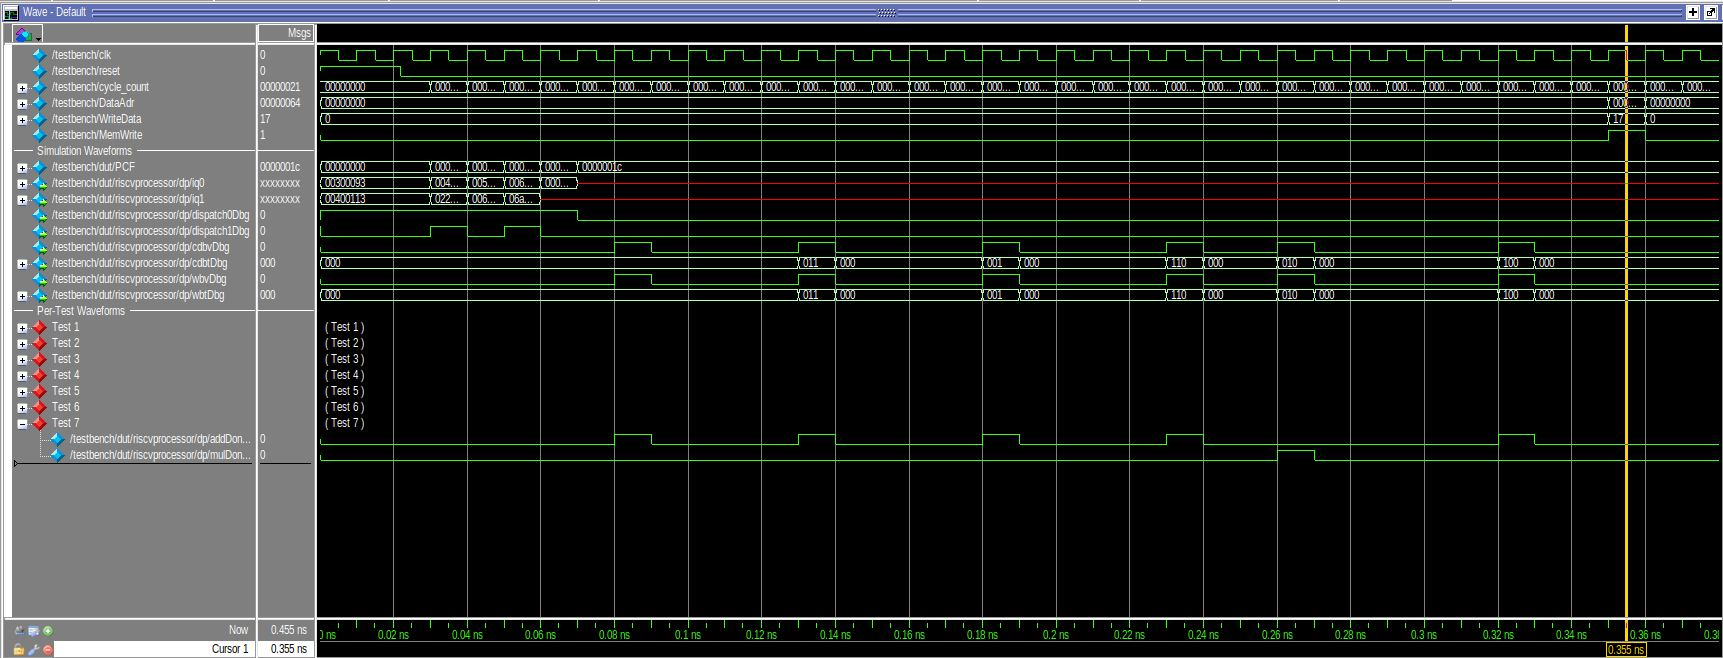
\includegraphics[width=0.95\textwidth]{images/test7_waveforms.png}
  \caption{Example baseline waveform capture (existing artifact).}
  \label{fig:wave_test7}
\end{figure}

\begin{figure}[!htbp]
  \centering
  \IfFileExists{images/rob01_waveforms.png}{%
    \includegraphics[width=0.95\textwidth]{images/rob01_waveforms.png}%
  }{%
    \fbox{\parbox{0.92\textwidth}{\centering
        \vspace{1.2cm}Insert waveform screenshot: \texttt{rob01\_waw\_order}\vspace{1.2cm}
      }}%
  }
  \caption{ROB01: WAW completion/commit ordering.}
  \label{fig:wave_rob01}
\end{figure}

\begin{figure}[!htbp]
  \centering
  \IfFileExists{images/rob03_waveforms.png}{%
    \includegraphics[width=0.95\textwidth]{images/rob03_waveforms.png}%
  }{%
    \fbox{\parbox{0.92\textwidth}{\centering
        \vspace{1.2cm}Insert waveform screenshot: \texttt{rob03\_beq\_taken} (flush/redirect)\vspace{1.2cm}
      }}%
  }
  \caption{ROB03: branch misprediction flush and redirect.}
  \label{fig:wave_rob03}
\end{figure}

\begin{figure}[!htbp]
  \centering
  \IfFileExists{images/rob04_waveforms.png}{%
    \includegraphics[width=0.95\textwidth]{images/rob04_waveforms.png}%
  }{%
    \fbox{\parbox{0.92\textwidth}{\centering
        \vspace{1.2cm}Insert waveform screenshot: \texttt{rob04\_misaligned\_trap} (exception to trap)\vspace{1.2cm}
      }}%
  }
  \caption{ROB04: precise exception and trap timing.}
  \label{fig:wave_rob04}
\end{figure}

\section{Conclusion}

Project 3 extends my Project 2 submission with a 16-entry Reorder Buffer that
cleanly separates out-of-order execution from in-order architectural commit.
The ROB entry index doubles as the rename tag, so CDB snoop logic in the
reservation stations needed only a tag-width change --- not a semantic one ---
to interoperate with the new commit model. Committing architectural register
writes and memory stores only at the ROB head removes the speculative-retire
problem that the earlier design could not have handled: predict-not-taken
branches now flush cleanly and a precise-exception trap on a misaligned
load/store cleanly halts the pipeline with older instructions fully retired
and younger instructions fully suppressed. A one-entry store buffer restores
the store-then-load-same-address behaviour that the move to commit-time
memory writes would otherwise break, without violating the ``no speculative
memory writes'' invariant. All eleven regression tests pass.

\end{document}
